\chapter{Rate Limiter}\label{ch:rate-limiter}

\resilienceMechanismChapterIntro{Rate Limiter}{proactive}


\section{Introduction}\label{sec:rate-limiter-introduction}

The Rate Limiter is a proactive resilience mechanism
that aims to control the rate at which requests are made to a service or resource.
By imposing a limit on the number of requests within a given time period,
the Rate Limiter helps to prevent overloading downstream services,
ensuring stability and availability~\cite{microsoft-rate-limiting-pattern}.

Advantages of using a Rate Limiter include~\cite{solo-io-rate-limiting, kong-rate-limiting}:

\begin{itemize}
    \item \textbf{Prevent malicious activities}: Rate limiting can help protect against brute force, denial-of-service, and distributed denial-of-service (DDoS) attacks, web scraping, and other malicious activities~\cite{cloudflare-rate-limiting};
    \item \textbf{Manage Resource Utilization}: By controlling the rate of requests, rate limiting helps to manage resource utilization, prevent resource starvation, and ensure that resources are available for all users following predefined SLAs (Service Level Agreements);
    \item \textbf{Prevent Abuse}: Stops users from monopolizing resources and prevents excessive or unnecessary requests, ensuring fair resource distribution and optimal network or server performance;
    \item \textbf{Improve User Experience}: Rate limiting reduces delays and enhances the responsiveness of the service for legitimate users, improving the overall user experience;
    \item \textbf{Reduce Costs}: Helps avoid extra costs associated with overloading resources, as limiting request rates reduces the demand on resources and prevents the need for additional capacity.
\end{itemize}

\subsection{API Gateway}\label{subsec:rate-limiter-api-gateway}

An API Gateway is a server or software application that acts as an intermediary between clients and backend services or microservices.
It serves as a single entry point for API calls, managing and routing them to the appropriate services, while also providing various functionalities to enhance security, performance, and usability.

One of the key features~\cite{api-gateway} of an API Gateway's traffic management is the implementation of rate limiting and throttling policies.
These policies control the rate of incoming requests and set rules and limits to regulate traffic, preventing the overloading of backend services.

\subsection{Relation To The Throttling Mechanism}\label{subsec:rate-limiter-throttling}

Rate limiting and throttling are closely related concepts often used interchangeably,
since both mechanisms control the rate of incoming requests to protect services from being overwhelmed, but they have distinct differences.
Rate limiting refers to the process of restricting the number of requests that can be made to a service within a given time period.
Throttling, on the other hand,
specifically adjusts the flow rate based on current system load.
Is typically used to ensure that high-priority requests are served first by delaying less critical ones.

To better illustrate the difference between these two concepts, consider the following analogy:
a rate limiter is like traffic lights that control the number of cars that can pass through an intersection within a certain time frame,
whereas throttling is like an adjustable hose nozzle that can be adjusted to control the flow of water, allowing more or less water to pass through based on the current water pressure.

\subsection{Semaphore}\label{subsec:rate-limiter-semaphore}

A semaphore is a synchronization primitive that restricts the number of simultaneous accesses to a shared resource
up to a specified limit.
Key characteristics and operations of a semaphore include~\cite{java-semaphore, oracle-multithreaded-programming-guide}:

\begin{itemize}
    \item \textbf{Permits}: The semaphore keeps track of available permits.
    Each permit represents a single unit of resource access that can be granted.
    Resource access may require multiple permits, depending on the use case;
    \item \textbf{Acquire}: This operation decreases the number of available permits by a given number.
    If no permits are available, the acquiring entity is blocked (in the case of threads) or suspended (in the case of coroutines) until a permit is released;
    \item \textbf{Release}: This operation increases the number of available permits by a given number.
    Since releasing permits possibly created conditions for other entities (waiting to acquire permits) to proceed, then the semaphore notifies them.
\end{itemize}

There are two main types of semaphores:
\begin{itemize}
    \item \textbf{Binary Semaphore}:
    This type has only two states: available (1 permit) and unavailable (0 permits).
    In literature, it is also misconceptionally known as a mutex (mutual exclusion lock),
    but differs in ownership rights.
    An acquired mutex can only be released by the entity that acquired it, while a semaphore can be signalled by any other entity.
    \item \textbf{Counting Semaphore}: This type can have a count greater than one, allowing multiple entities to acquire permits up to a specified limit.
    It is used for managing access to a resource pool.
\end{itemize}

In the context of rate limiting, a semaphore can be used to control the rate of incoming requests by granting or denying access based on the availability of permits.

\subsection{Rate Limiting Algorithms}\label{subsec:rate-limiter-algorithms}

There are several algorithms that can be used to implement rate limiting, each with benefits and drawbacks to consider.
Alas,
the choice of algorithm depends on the specific requirements of the system and the challenges it faces
(i.e., implementation on a single server or distributed system, handling bursty traffic, etc.)
~\cite{medium-rate-limiting-algorithms,nordic-apis-rate-limiting-algorithms}:

\subsubsection{Token Bucket}\label{subsubsec:token-bucket-algorithm}

This algorithm is used in packet-switched and telecommunications networks
to check data transmissions against defined limits on bandwidth and burstiness
(a measure of unevenness or variations in traffic flow).
The token bucket algorithm is based on the concept of a bucket that holds tokens,
where each token represents a unit of data or a permit to transmit data.
The key features of the token bucket algorithm include:

\begin{itemize}
    \item Has a fixed capacity (maximum number of tokens it can hold) and a refill rate (tokens added per unit of time);
    \item Tokens are added to the bucket at a constant rate, up to the maximum capacity;
    \item When a packet arrives, it must acquire a token from the bucket to proceed;
    \item If no tokens are available, the packet is considered non-conformant and may be dropped or delayed.
\end{itemize}

Provides a variable request rate and is suitable for handling bursts of requests,
as long as the bucket has enough tokens to accommodate them.
This algorithm can be implemented by a semaphore with no release operation, as the permits are automatically refilled at a constant rate.

\subsubsection{Leaky Bucket}\label{subsubsec:leaky-bucket-algorithm}

The leaky bucket algorithm is another rate limiting algorithm used in network traffic management, and is conceptually similar to the token bucket algorithm.
It is analogous to a bucket with a hole in the bottom that leaks water at a constant rate.
This algorithm's advantage is that it smooths out bursts of requests and processes them at an approximately constant rate.
This way smoothing out traffic bursts and preventing congestion.

However,
a burst of traffic can starve more recent requests from being processed
while providing no guarantee that requests get processed in a fixed amount of time.
Additionally, if you load balance servers for fault tolerance or increased throughput,
you must use a policy to coordinate and enforce the limit between them~\cite{kong-rate-limiting}.

\subsubsection{Fixed Window Counter}\label{subsubsec:fixed-window-counter-algorithm}

The fixed window counter algorithm essentially counts the number of requests made within discrete,
fixed time intervals.

The key features of the fixed window counter algorithm include:

\begin{itemize}
    \item Requests are counted within a fixed time window (e.g., 1 second, 1 minute);
    \item When a request is made, the counter is incremented;
    \item If the counter exceeds the rate limit, the request is rejected;
    \item The counter is resetted at the beginning of each time window.
\end{itemize}

The fixed window counter algorithm is easy to implement but can lead to bursty traffic patterns, as requests are not evenly distributed within the time window.
For example, if the rate limit is 5 requests per minute and a user makes 5 requests at the end of the time window, they can circumvent the limit by making 5 more requests at the beginning of the next time window, effectively doubling the allowed requests as shown in Figure~\ref{fig:fixed-window-counter-problem}.

\begin{figure}[!htb]
    \centering
    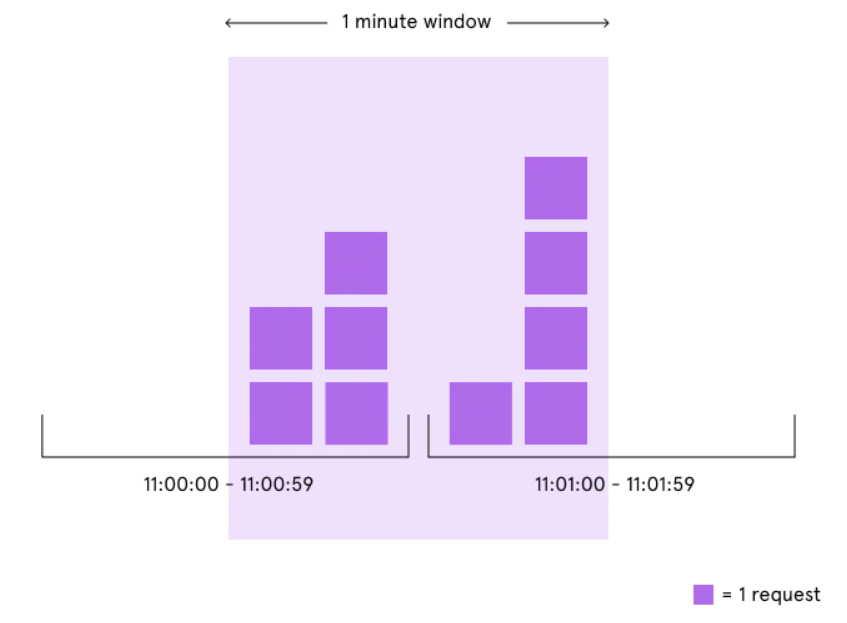
\includegraphics[width=0.5\textwidth]{../figures/06_fixed-window-counter-problem}
    \caption{Fixed Window Counter Problem.
    Retrieved from~\cite{medium-rate-limiting-algorithms}}.
    \label{fig:fixed-window-counter-problem}
\end{figure}

Additionally, the fixed window counter algorithm can lead to a stampeding effect,
where previously rejected requests are retried simultaneously when the time window resets.
This effect can cause spikes in traffic and overload the system, especially when dealing with a large number of clients.

\subsubsection{Sliding Window Log}\label{subsubsec:sliding-window-log-algorithm}

The sliding window log algorithm maintains a continuous record of requests over a rolling time period.

Key features of the sliding window log algorithm include:

\begin{itemize}
    \item Tracks requests within a continuously moving window (e.g., last 60 seconds);
    \item Maintains a log of timestamps for each request in the sliding window;
    \item Checks the log to count the number of requests in the current window whenever a new request is made;
    \item Helds the request if the count exceeds the rate limit;
\end{itemize}

Unlike the fixed window counter algorithm,
the sliding window log algorithm provides a more accurate representation of request rates over time,
and it does not suffer from the boundary conditions of fixed windows.
However, it can be memory-intensive, as it stores a timestamp for each request, and computationally expensive,
as each request requires summing up prior requests, which may not scale well with a large number of requests.

\subsubsection{Sliding Window Counter}\label{subsubsec:sliding-window-counter-algorithm}

The sliding window counter algorithm combines the efficiency of the fixed window approach with the accuracy of the sliding log method, providing smooth rate limiting over a rolling time period.

Key features of the sliding window counter algorithm include:

\begin{itemize}
    \item Divides the time window into smaller fixed segments (e.g., 1-second segments within a 60-second window);
    \item Tracks the count of requests for each segment;
    \item Calculates the total number of requests in the current window by summing the counts of the relevant segments;
    \item Rejects the request if the total number of requests within the sliding window exceeds the rate limit;
    \item Continuously updates the sliding window by shifting the segments as time progresses, ensuring an accurate count for the current window.
\end{itemize}

This hybrid approach smooths out traffic bursts
by weighting the previous window’s request rate based on the current timestamp,
similar to the sliding log method
(e.g., if the current window is 25\% through, the previous window's count is weighted by 75\%).
The sliding window counter algorithm provides the flexibility to scale rate limiting with good performance, avoiding the starvation problem of the leaky bucket and the burstiness of fixed window implementations~\cite{kong-rate-limiting}.

\subsection{Rate Limit Exceeded}\label{subsec:rate-limiter-exceeded}

Rate limiting algorithms can deploy different strategies for handling requests when the rate limit is exceeded.
The most common approaches include:

\begin{itemize}
    \item \textbf{Reject}: Immediately deny the request and return an error response message (e.g., throwing an exception,
    returning an HTTP status code such as 429 - Too Many Requests), indicating that the rate limit has been reached;
    \item \textbf{Wait}: Place the request in a queue to be processed later when the rate limit allows, ensuring that the request is not lost and will eventually be handled;
    \item \textbf{Both}: Combine the previous two approaches by placing the request in a queue with a timeout.
    If the request cannot be processed within the timeout period, it is rejected.
\end{itemize}

\subsection{Distribution}\label{subsec:rate-limiter-distribution}

In a distributed system,
rate limiting can be challenging due to the need
to maintain consistency across multiple instances of the rate-limited service.
One simple way to enforce the limit is
to set up sticky sessions in your load balancer so that each consumer gets sent to exactly one node.
However, this approach has several disadvantages,
including a lack of fault tolerance and scaling problems when nodes get overloaded~\cite{kong-rate-limiting}.

A better option is to use a centralized data store (e.g., a database) to store the rate limit state,
allowing all instances of the service to access and update the state in a consistent manner.
This approach has the disadvantage
of introducing additional latency due to network communication with the data store and race conditions when
multiple instances try to update the state simultaneously.

A naive approach to distributed rate limiting is to use a `get-then-set' approach,
where the rate limit state is read from the data store, incremented, and then written back.
The issue with this model is that during the read-increment-store cycle, additional requests may arrive, leading each to attempt storing an incremented counter value, potentially resulting in an invalid (lower) counter value. This can enable consumers to send a high rate of requests, bypassing rate limiting controls~\cite{kong-rate-limiting}.

A few solutions arise to address these challenges:

\begin{itemize}
    \item \textbf{Locks}: Prevent concurrent access to the rate limit state by using locks to synchronize access.
    However, locks can introduce performance bottlenecks in high-concurrency scenarios;
    \item \textbf{Atomic Operations}:
    Use atomic operations provided by the data store to increment and check counters efficiently.
    Using more of the `set-then-get' approach can reduce the number of round trips to the data store;
\end{itemize}

To minimize latency introduced by using a centralized data store,
rate limit checks can be performed locally in memory with an eventually consistent model as shown in Figure~\ref{fig:distributed-rate-limiting-centralized}.
Each node periodically syncs with the centralized store,
pushing counter-increments and retrieving updated values (to update the local cache).
\textit{\enquote{The periodic rate at which nodes converge should be configurable. Shorter sync intervals will result in less divergence of data points when spreading traffic across multiple nodes in the cluster (e.g., when sitting behind a round robin balancer). Whereas longer sync intervals put less read/write pressure on the datastore and less overhead on each node to fetch new synced values}}~\cite{kong-rate-limiting}.

\begin{figure}[!htb]
    \centering
    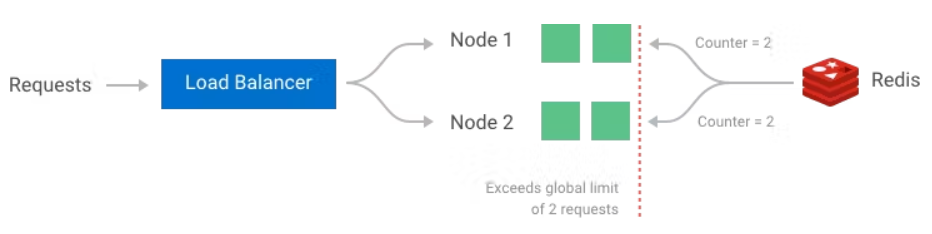
\includegraphics[width=0.8\textwidth]{../figures/06_distributed_rate_limiting}
    \caption{Distributed Rate Limiting with a Centralized Data Store.
    Retrieved from~\cite{kong-rate-limiting}}.
    \label{fig:distributed-rate-limiting-centralized}
\end{figure}

\section{Implementation Aspects}\label{sec:rate-limiter-implementation}

TODO(what aspects went to the design and implementation aspects were considered)

\subsection{Available Solutions}\label{subsec:rate-limiter-solutions}

Resilience4j provides two rate limiting implementations:
\begin{itemize}
    \item \texttt{AtomicRateLimiter}: A rate limiter that uses an atomic counter to control the rate of requests.
    It is based on the token bucket algorithm and can be configured with a refresh period to refill the bucket.
    \item \texttt{SemaphoreBasedRateLimiter}:
    A rate limiter that uses a semaphore to control the rate of requests and a scheduler to refill the semaphore.
\end{itemize}

Polly provides a thin layer over the .NET \texttt{System.Threading.RateLimiting}~\cite{microsoft-rate-limiting-dotnet} package,
which includes the following rate limiting implementations:
\begin{itemize}
    \item \texttt{TokenBucketRateLimiter}: Implements a token bucket algorithm to limit the rate of requests. Tokens are added to the bucket at a steady rate, and each request consumes a token. If no tokens are available, the request is denied or queued until tokens become available;
    \item \texttt{FixedWindowRateLimiter}: Uses a fixed window algorithm where requests are counted within fixed time intervals (windows);
    If the number of requests exceeds the limit for a window, further requests are denied until the next window.
    \item \texttt{SlidingWindowRateLimiter}: Employs a sliding window algorithm to provide smoother rate limiting by tracking requests over a rolling time period, rather than fixed intervals. This helps in avoiding bursts of traffic that occur at the boundary of fixed windows;
    \item \texttt{ConcurrencyLimiter}: Limits the number of concurrent requests. It uses a semaphore to restrict the number of simultaneous operations, ensuring that only a certain number of requests can be processed concurrently;
    \item \texttt{PartionedRateLimiter}: Allows rate limiting based on different keys or partitions.
    This is useful when you want to apply different rate limits to different groups of requests or users.
    \item \texttt{ChainedPartitionedRateLimiter}:
    Chains multiple rate limiters together to provide a cascading rate limiting strategy.
    If one rate limiter fails, all previously acquired permits are released, ensuring atomicity in rate limiting decisions.
\end{itemize}

Additionally,
the package also provides options
to configure the rate limiter with custom policies for handling rate limit exceeded scenarios,
the most notable being the queue processing strategy
(e.g., newest first, oldest first, etc.) and auto replenishment of permits (i.e., if disabled, the replenishment must be done manually).

Polly also provides a \texttt{LockFreeTokenBucketRateLimiter} implementation
that uses a lock-free algorithm to manage the token bucket,
improving performance in high-throughput scenarios.
Furthermore, the \texttt{RateLimiter} strategy can be used in two flavors: to control inbound load via a rate limiter and to control outbound load via a concurrency limiter.


\subsection{Components}\label{subsec:rate-limiter-components}

\begin{itemize}
    \item \textbf{Semaphore}: To manage the acquisition and release of permits for requests in a synchronized way.
    This is used to control access to the shared resources (e.g., the rate-limited service) and is conceptually similar to the token bucket algorithm, where a token represents a permit;
    \item \textbf{Queue}: To hold requests when the rate limit is exceeded;
    \item \textbf{Centralized Data Store}: The \texttt{Queue} and \texttt{Semaphore} components require a centralized state management (e.g., a database) to ensure consistency across multiple, possibly load-balanced, instances of the rate-limited service.
\end{itemize}


\section{Configuration}\label{sec:rate-limiter-configuration}

TODO(all mechanisms configuration should be after the implementation description, alter this)
